\documentclass[12pt]{article}
\usepackage{amsmath}
\usepackage{amssymb}
%\usepackage{hyperref}
\usepackage{epsfig,graphicx,amsmath}
\usepackage{amsfonts}
\usepackage{enumerate}
\usepackage{amsfonts}
\usepackage{amssymb}
\usepackage{amsthm}


\newcommand{\mb}[1]{\mbox{\boldmath$#1$}}
\newcommand{\p}{\partial}
\newcommand{\ds}{\displaystyle}
\newcommand{\beq}{\begin{eqnarray}}
\newcommand{\beqq}{\begin{eqnarray*}}
\newcommand{\eeq}{\end{eqnarray}}
\newcommand{\eeqq}{\end{eqnarray*}}
\newcommand{\eps}{\varepsilon}
\newcommand{\erf}{\mbox{erf}}
\newcommand{\erfi}{\mbox{erfi}}
\newcommand{\Ei}{\mbox{Ei}}
\newcommand{\x}{\mbox{\boldmath$x$}}
\newcommand{\Aa}{\mbox{\boldmath$A$}}
\newcommand{\rr}{\mbox{\boldmath$r$}}
\newcommand{\As}{\mbox{\boldmath$a$}}
\newcommand{\y}{\mbox{\boldmath$y$}}
\newcommand{\z}{\mbox{\boldmath$z$}}
\newcommand{\J}{\mbox{\boldmath$J$}}
\newcommand{\ET}{\mbox{\boldmath$\eta$}}
\newcommand{\n}{\mbox{\boldmath$n$}}
\newcommand{\X}{\mbox{\boldmath$X$}}
\newcommand{\Y}{\mbox{\boldmath$Y$}}
\newcommand{\Yy}{\mbox{\boldmath$y$}}
\newcommand{\Z}{\mbox{\boldmath$Z$}}
\newcommand{\w}{\mbox{\boldmath$w$}}
\newcommand{\vv}{\mbox{\boldmath$v$}}
\newcommand{\bb}{\mbox{\boldmath$b$}}
\newcommand{\Bb}{\mbox{\boldmath$b$}}
\newcommand{\B}{\mbox{\boldmath$B$}}
\newcommand{\ALPHA}{\mbox{\boldmath$\alpha$}}
\newcommand{\aaa}{\mbox{\boldmath$a$}}
\newcommand{\C}{\mbox{\boldmath$C$}}
\newcommand{\SSigma}{\mbox{\boldmath$\Sigma$}}
\newcommand{\mmu}{\mbox{\boldmath$\mu$}}
\newcommand{\IIm}{\mbox{\boldmath$I_m$}}
\newcommand{\mean}[1]{\langle #1\rangle}
\newcommand{\diffunit}{$\mu$m$^2$.s$^{-1}$}
\newcommand{\Li}{\mbox{Li}}
\newcommand{\thet}{\mbox{\boldmath$\theta$}}
\newcommand{\intR}{\int\limits_{\mathbb{R}}}
\newcommand{\intRm}{\int\limits_{\mathbb{R}^m}}
\newcommand\norm[1]{\left\lVert#1\right\rVert}
%\definecolor{red}{rgb}{1,0,0}

\usepackage{color}
\usepackage{float}
\begin{document}	
	\title{Results \& Material and methods}
	\author{Ofir Shukron \& David Holcman}
	\maketitle
	
	\section{Result section}
	To estimate the nucleosome reorganization following DNA damages, we have
	constructed a mathematical model, where redistribution can be due either to chromatin de-
	compaction or nucleosome sliding along the chromatin or both of them. We
	have used the model to assess the relative contribution of these two processes
	to the total DNA and nucleosome signal loss from a region of interest (ROI),
	a quantity which is inaccessible experimentally.
	
	The model (presented in Material and methods) follows the DNA, $D(u)$,
	and nucleosome, $H(u)$, fraction of signal loss from the ROI as a function of
	the UV dose, $u$. We have used the measured H3.3 and DNA signal loss to
	calibrate parameters of nucleosome and DNA models respectively (Fig. 3A-
	D). Using the calibrated models we have found that the relative contribution
	of nucleosome sliding to the total signal loss in the ROI is monotonically
	decreasing from 75\% to 70\% for nucleosomes and 51\% to 40\% for DNA loss,
	as the UV dose increases from 5 to 100 msec. The remaining percentages are
	attributed to chromatin expansion and de-compaction (see Figure \ref{fig:relatiiveContributionToLoss}).
	
	\begin{figure}[H]
		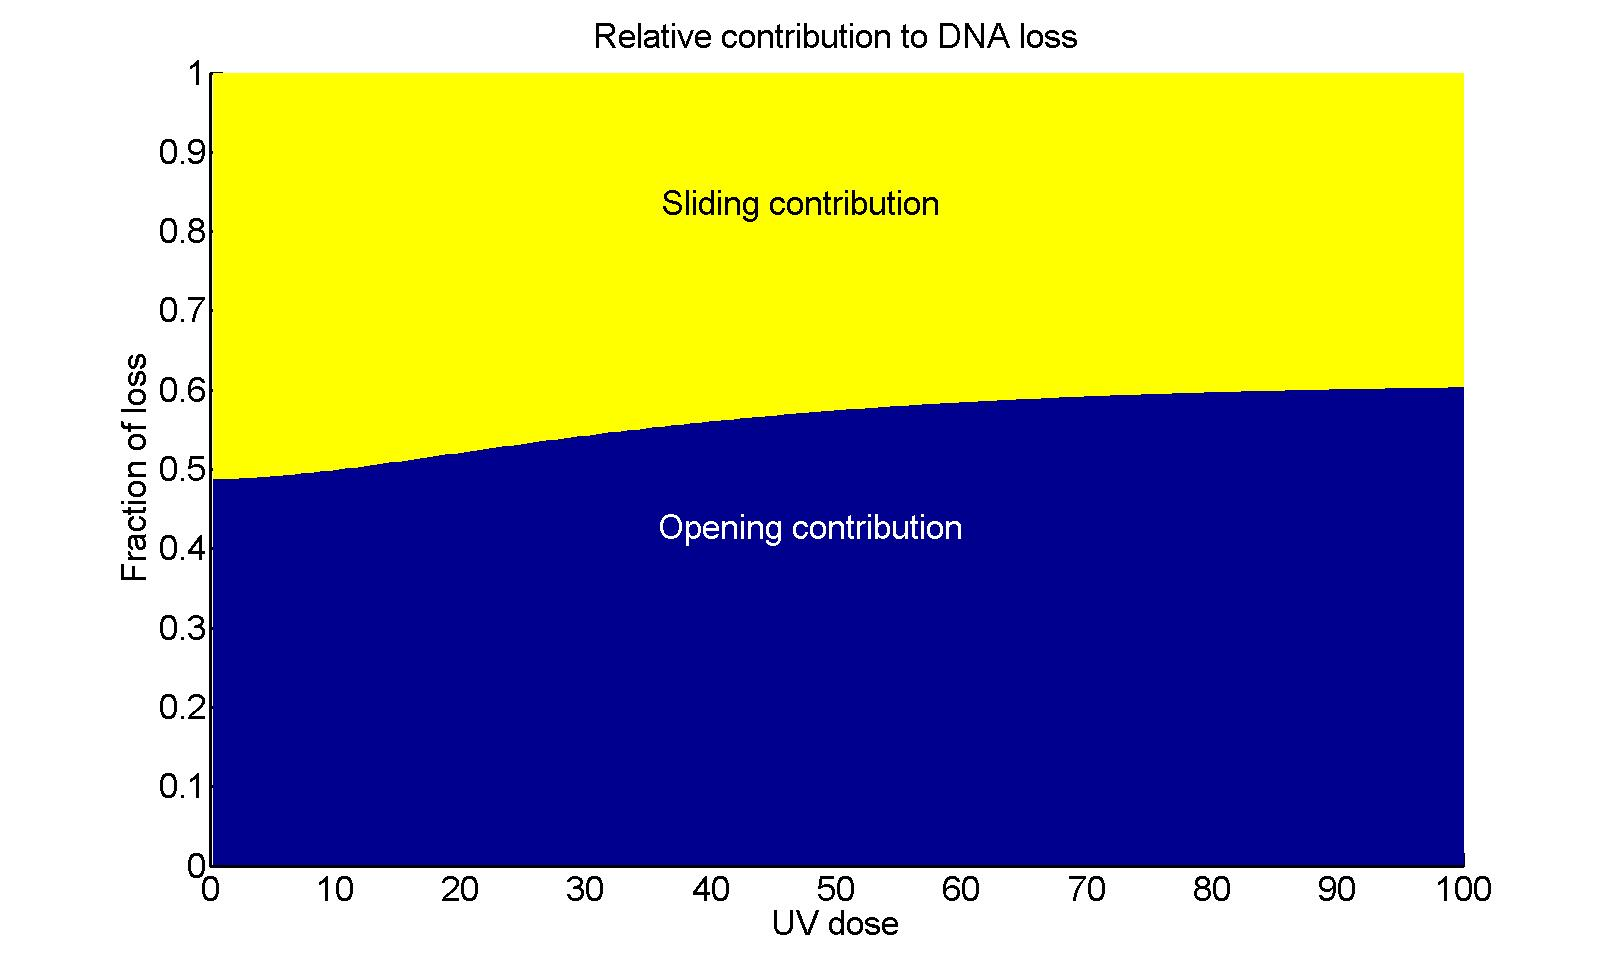
\includegraphics[width=0.5\linewidth, height=0.3\textheight]{relatiiveContributionToDNALoss}
		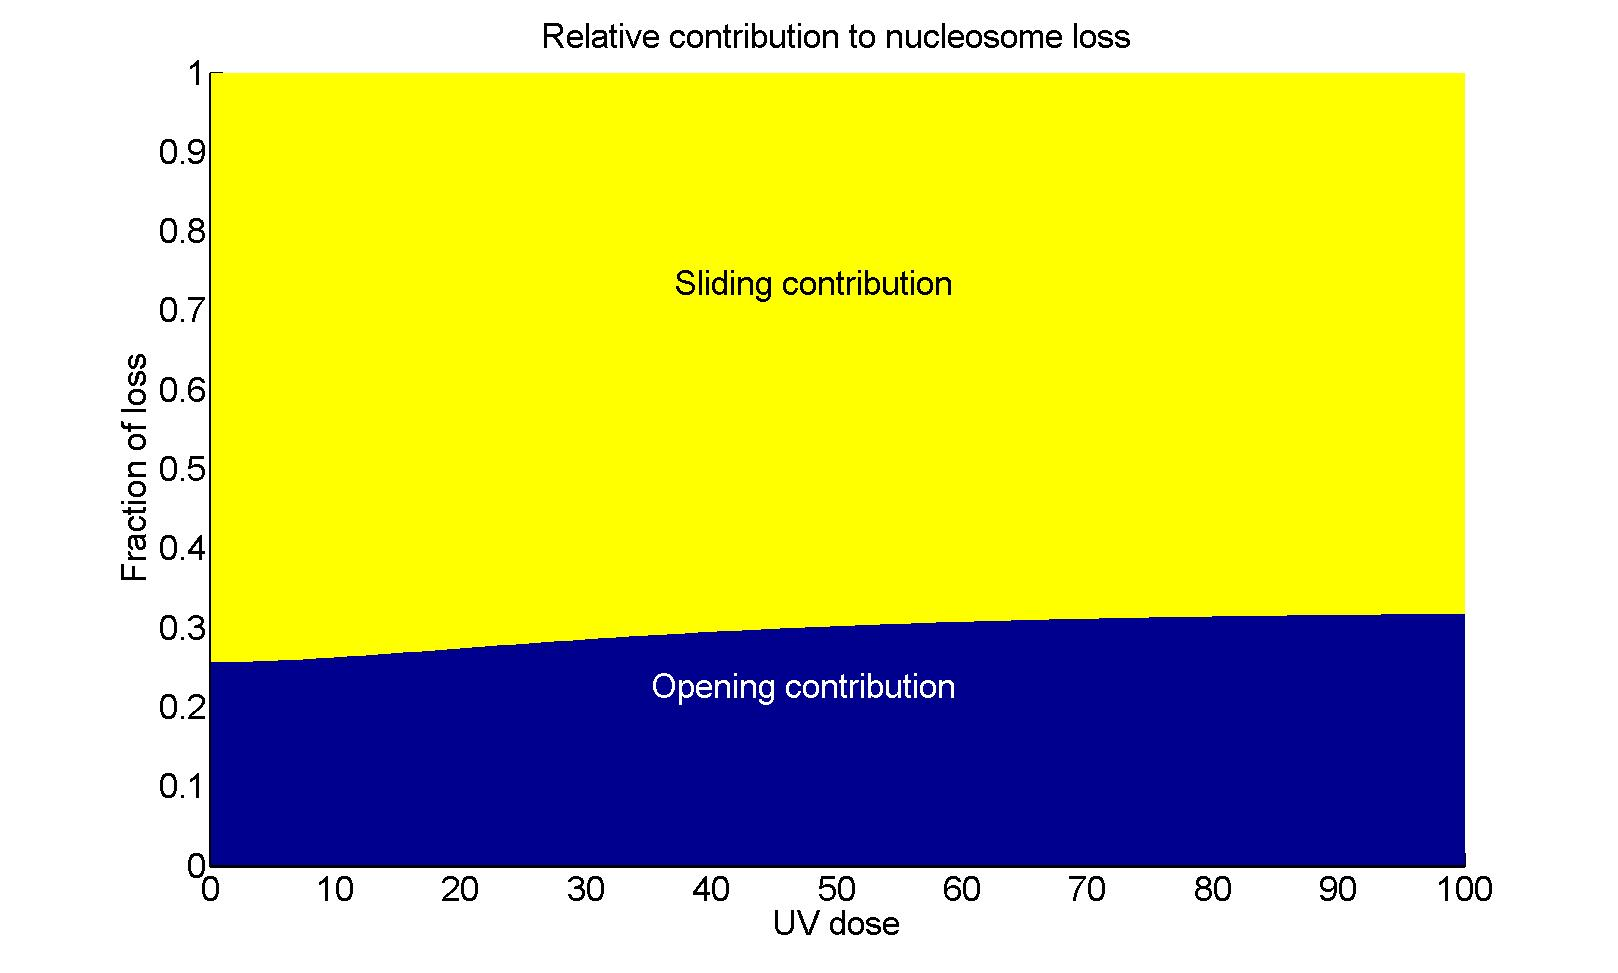
\includegraphics[width=0.5\linewidth, height=0.3\textheight]{relativeContributionToHistoneLoss}
		\caption{\textbf{Relative contribution of chromatin opening and nucleosome sliding to DNA (left) and histone (right) loss}. Sliding contribution is monotonically decreasing with UV dose for both DNA and nucleosome signals. The increase in chromatin opening contribution is due to the increase in chromatin reorganization following high dosages of UV, which is responsible for the majority of signal loss.}
		\label{fig:relatiiveContributionToLoss}
	\end{figure}
	
 \section{ Material and methods: Modeling nucleosomes and DNA redistribution following UV
		damages} 
	
	We present here a model for nucleosomes and DNA re-organization following
	UV damages. The cascade of events leading to tagged DNA and nucleosomes'
	redistribution, results in signal extrusion from a region of interest (ROI) up
	to a maximal loss, measured 15 minutes post UV-C.
	
	\subsection{Dynamics of nucleosomes following UV damages
		in the region of interest}
	
	Following the experimental protocol, a two-dimensional circular initial damage region (IDR), induced by the UV laser beam, is centered around the focal point (origin of the coordinates) with a fixed area of $A_0$. Following
	laser induction with a UV dose $u$, the tagged damage region expands radially outward and reaches its maximal area of $A(u)$ after 15 minutes. At the end of expansion, the circular region is defined
	as the ROI, in which DNA and nucleosome signal is measured at
	time 0 and 15 minutes. The fraction of signal loss is calculated for DNA and nucleosomes as
	\begin{equation}
	\frac{signal_0-signal_{15}}{signal_0}
	\end{equation}	
	where $signal_0$ and $signal_{15}$ are the DNA or nucleosome signal at time 0 and 15 minutes respectively. 
	
	We assume that the loss of DNA and nucleosomes signal post UV-C is due
	to two mechanisms: the first is chromatin expansion, and the second is nucleosomes sliding along the chromatin. For chromatin expansion, recruitment and
	binding of repair factors to damaged DNA causes chromatin de-compaction, and cross-links break [ref] to enable repair factor access to damaged DNA. Because the majority of damages are inflicted around the laser's focal point, the accumulation of repair factors will generate a pushing force on surrounding chromatin in a radial outward direction. As a result of the pushing force, DNA and nucleosome will be extruded from the ROI in equal proportions. 
	
	An additional loss of nucleosome signal is caused by the mechanism of nucleosome sliding. Repair proteins slide nucleosomes from damaged position on the DNA away from high concentration of DNA damages. Each nucleosome sliding over damaged positions on the DNA displaces the tagged damages
    spatially in the general direction of the ROI boundary. Additionally, with each nucleosome sliding, the damages in the damage region are exposed, and repair factors are recruited to bind to them.   
    expansion of the IDR and signal loss from the ROI.

    In-line with the description above, we construct a model representing
	signal loss 15 minutes post UV-C. We do not specifically take into account the
	mechanism of signal loss in time and only present the steady-state equations
	for signal loss as a function of the UV dose.
	
	\subsection{Steady-state equations describing DNA and nucleosome loss}
	
	We assume an initial uniform distribution of both DNA and nucleosome in
	the IDR and its vicinity. such that the amount of DNA and nucleosomes in
	the IDR is proportional to its area. We define the number of nucleosomes leaving the IDR 15 minutes post UV-C as $N_T(u) = N_P(u) + N_S(u)$,
	with $N_S(u)$ and $N_P(u)$ the number of nucleosomes sliding and pushed out
	of the IDR, respectively. Nucleosomes pushed out of the IDR are associated
	with undamaged DNA, therefore we set $D_p(u)/A_0 = N_P(u)/N_0$ to represent this
	quantity. The IDR and the ROI are considered to be two-dimensional concentric circular regions, characterized by an area $A_0$ and $A(u)$ respectively,
	with $A(u) > A_0$, for all $u$ values. We shall now compute the fraction of
	DNA loss (resp. nucleosomes) $D(u)$ (resp. $H(u)$) in the ROI 15 minutes
	post UV-C.
	
	By construction, DNA signal loss is given by the ratio of the amount of
	DNA in the annulus between the IDR and the ROI plus the nucleosomes
	pushed out of the IDR to the total amount of signal in the ROI. Nucleosome signal loss is calculated as the sum of the nucleosomes that have been
	translocated with the DNA plus the ones that are sliding out, resulting in
	the following formulas
	\begin{equation}\label{eq:DNAstst}
	D(u) = \frac{(A(u)/A_0)-1 + (D_P(u)/A_0)}{A(u)/A_0}	
	\end{equation}
	
	\begin{equation}\label{eq:nucleosomeStst}
	H(u) = D(u) + \frac{N_S(u)/N_0}{A(u)/A_0}	
	\end{equation}
	
	In order to evaluate the functions above, we will now construct models
	for the functions $A(u)$ and $N_T(u)$. The increase of DNA damages with UV
	dose is thought of as governing the dynamics of both nucleosome and DNA
	signal loss. Therefore, we start our construction with a description of the
	accumulation of damages $T(u)$ in the IDR, and derive the function $N_T(u)$
	and $A(u)$ from it
	
	\subsection{Deriving the number of damages $T(u)$}
	
	We will derive the equation describing accumulation of damages on a radial
	cross-section of the IDR and then expand it to the whole IDR. We assume
	here that the rate of accumulating DNA damages along the radius of the
	IDR, $T_r(u)$, with increasing UV dose in the IDR is increasing proportional
	to the undamaged DNA in that cross-section.
	
	\begin{equation*}
	\frac{dT_r(u)}{du} = k_t(T_{max} - T_r(u))
	\end{equation*}	
	with $k_t$ the rate constant, and $T_{max}$ the maximal number of damages possible
	along the radius. Using the initial condition $T_r(0) = 0$, the solution is
	
	\begin{equation*}
	T_r(u) = T_{max}(1-\exp(−k_tu))
	\end{equation*}
	
	Expanding this equation to describe damages in a two-dimensional IDR, we
	obtain
	\begin{equation}\label{eq:damagesIDR}
	T(u) = \pi T_{max}^2 (1-\exp(−k_tu))^2
	\end{equation}
	
	We assume no two damages can occur in the same position on the DNA,
	hence we can treat the quantity
	\begin{equation*}
	T(u)/(\pi T_{max}^2)
	\end{equation*}
	as the fraction of chromatin length in the IDR which is damaged, or as the
	DNA damage-coverage percentage.
	
	\subsection{Deriving the functions describing loss of nucleosome from the IDR and the ROI expansion}
	We now turn to construct a model for the total number of nucleosomes $N_T(u)$
	leaving the IDR and subsequently being pushed out of the ROI, as a function
	of the UV dose. Although the exact mechanism by which nucleosomes are
	lost is not known, we assume here that the number of nucleosomes leaving
	the ROI is composed of two contributions, one due to nucleosomes pushed
	out of the IDR, and the second due to nucleosome sliding to expose damaged
	DNA positions and facilitate efficient repair.
	
	The nucleosomes occupy a length of the chromatin proportional to $N_0-
	N_T(u)$, whereas chromatin damage coverage is proportional to $T(u)$. Therefore, in the first-order approximation, the dynamics of $N_S(u)$ is given by the multiplication
	\begin{equation*}
	\frac{dN_S(u)}{du} = k_s\frac{(N_0-N_T(u))}{\pi T_{max}^2}\frac{dT(u)}{du}	
	\end{equation*}
	with $k_s$ the rate constant. Due to the accumulation of repair factors around
	damaged DNA, a pushing force acts on the surrounding undamaged DNA in
	the IDR. The rate nucleosomes are being pushed out of the IDR is considered
	to be proportional to the fraction of DNA damaged occurring due to small amount of
	UV dose, minus the fraction out of it which slides out
	
	\begin{equation*}
    \frac{dN_P(u)}{du}=k_p\left(\frac{(N_0-N_T(u))-k_s(N_0-N_T(u))}{\pi T_{max}^2}\right)\frac{dT(u)}{du}
	\end{equation*}
	
	The dynamics of $N_T(u)$ is obtained by adding equations 6 and 7. Using
	the initial condition $N_T(0) = 0$, we can solve for $N_T(u)$ to have
	\begin{equation}\label{eq:totalNucleosomeLossIDR}
	N_T(u) = N_0\left[1-\exp\left(-\frac{k_p(1-k_s)+k_s}{\pi T_{max}^2}T(u)\right)\right]
	\end{equation}
	
	Therefore, 
	\begin{equation}\label{eq:nucleosomePush}
	N_P(u) = \left(1-\frac{k_s}{k_p(1-k_s)+k_s}\right)N_T(u)
	\end{equation}
	\begin{equation}\label{eq:nucleosomeSlide}
	N_S(u) = \left(\frac{k_s}{k_p(1-k_s)+k_s}\right)N_T(u)
	\end{equation}
	with $k_s$ and $k_p$ constants describing the rate of nucleosome depletion from
	the ROI due to sliding and pushing respectively.
	
	Next, we model the dynamics of the ROI area $A(u)$ with increasing UV
	dose. For this end, we consider the ROI expansion to be affected by two
	additive mechanisms originating from the IDR: one is chromatin opening or
	de-compaction, and the other is nucleosome sliding. The two contributions
	are inherent in the equation for $N_T(u)$, therefore
	
	\begin{equation*}
	\frac{dA(u)}{du}=k_a\frac{dN_T(u)}{du}=k_a\left(\frac{dN_P(u)}{du}+\frac{dN_S(u)}{du}\right)
	\end{equation*}
	where $k_a$ is the rate constant. Using the initial condition $A(0) = A_0$, we find
	\begin{equation}\label{eq:areaROI}
	A(u) = A_0+ k_aN_0\exp\left(-\frac{(k_p(1-k_s)+k_s)}{\pi T_{max}^2}T(u)\right)
	\end{equation}
	where $A_0$ represents the size of the IDR even in the absence of UV induction.
	
	We can now substitute equations \eqref{eq:nucleosomePush}, \eqref{eq:nucleosomeSlide} and \eqref{eq:areaROI} into the steady-state equations \eqref{eq:DNAstst} and \eqref{eq:nucleosomeStst} to get the expressions for $D(u)$ and $H(u)$. Using the relation $D_p(u)/A_0 = N_p(u)/N_0$, we present the result in terms of $N_T(u)$			
	\begin{equation}\label{eq:DNALoss}
	D(u) = \frac{\frac{N_T(u)}{N_0}\left(\frac{k_p(1-k_s)}{k_p(1-k_s)+k_s}-\frac{k_aN_0}{A_0}\right)+\frac{k_aN_0}{A_0}}{1+\frac{k_aN_0}{A_0}\left(1-\frac{N_T(u)}{N_0}\right)}
	\end{equation}
	\begin{equation}\label{eq:nucleosomeLoss}
		H(u) = \frac{\frac{N_T(u)}{N_0}\left(1-\frac{k_aN_0}{A_0}\right)+\frac{k_aN_0}{A_0}}{1+\frac{k_aN_0}{A_0}\left(1-\frac{N_T(u)}{N_0}\right)}
	\end{equation}
	
	\subsection{Parameter fit for $D(u)$ and $H(u)$}\label{subsection:parameterFit}
	We now use equations \eqref{eq:DNALoss}  and \eqref{eq:nucleosomeLoss} to fit the experimental data. We simultaneously fit equations \eqref{eq:DNALoss}  and \eqref{eq:nucleosomeLoss} to the H3.3 and DNA loss data, with the goal of maximizing the $R^2$ of both equations. Excluding the measurement at 5 msec, and using classical fitting procedure, we find
	\begin{equation*}
	k_t = 0.037, \quad k_s = 0.35,\quad k_p = 0.24, \quad \frac{k_aN_0}{A_0} = 0.46
	\end{equation*}
	with $R^2 = 0.93$ and $R^2 = 0.96$ for DNA and nucleosome loss fit respectively.
	
	
\begin{figure}[H]
\centering
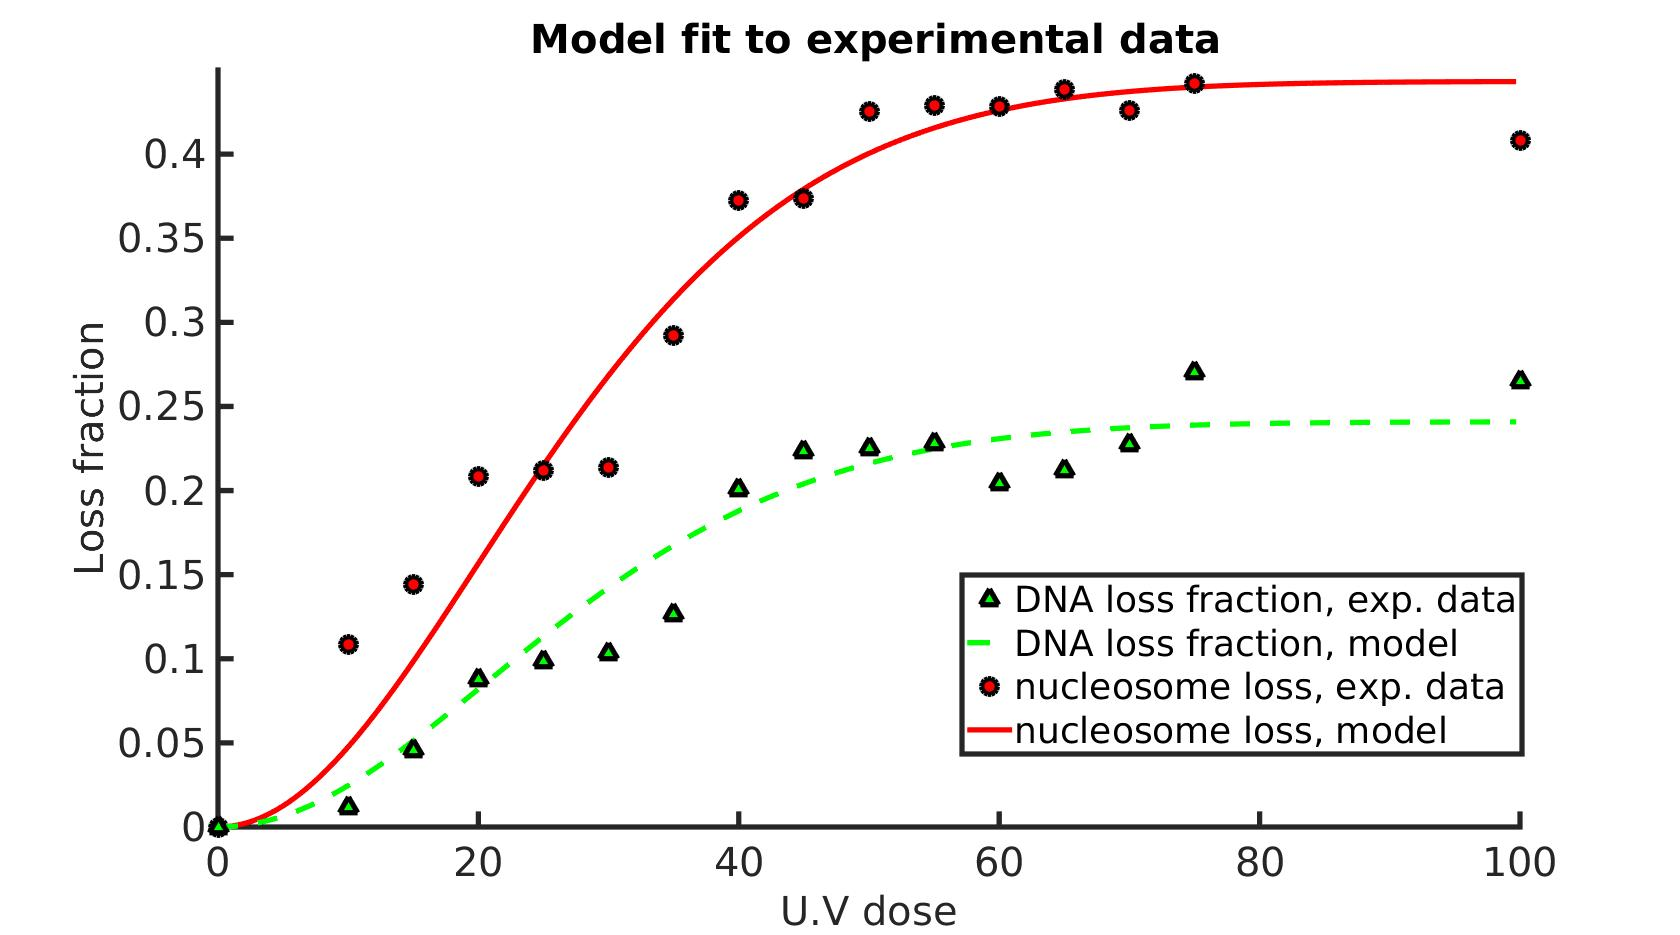
\includegraphics[width=0.5\linewidth, height=0.3\textheight]{histoneAndDnaVsUvDoseModelFit}
\caption{\textbf{Histone (red) and DNA (green) loss: experimental data
	for nucleosomes (circle) and DNA (triangles) versus model curves
	(continuous and dashed, respectively)}. Parameter values are obtained
	by simultaneously fitting equations\eqref{eq:DNALoss}  and \eqref{eq:nucleosomeLoss} to the experimental data with
	the goal of maximizing the $R^2$. The resulting curves show $R^2 = 0.96$ and
	$R^2 = 0.93$ for nucleosome and DNA loss, respectively.}
\label{fig:histoneAndDnaVsUvDoseModelFit}
\end{figure}

\subsection{Relative contribution of opening and sliding to DNA
	and nucleosome signal loss}

Using the calibrated model in equation equations \eqref{eq:DNALoss}  and \eqref{eq:nucleosomeLoss}, we now calculate the
relative contribution of chromatin opening and nucleosome sliding to the
total loss of DNA and nucleosomes. The sliding contribution refers to all loss
caused by either directly sliding nucleosome out of the IDR or as the effect
nucleosome sliding has on pushing chromatin out of the IDR by operations
of repair factors. Chromatin opening contribution refers to all signal loss
caused by chromatin remodeling, which causes expansion of the IDR and
subsequent loss of signal from the ROI.

We start by dividing the equation describing the ROI expansion into the
two sub-mechanisms of signal loss

\begin{equation*}
A(u) = A_P(u) +A_S(u)
\end{equation*}
with $A_P(u)$ the area attributed to chromatin opening, and $A_S(u)$ to nucleosome sliding. Subtracting the sliding contribution from the ROI expansion
in equation \eqref{eq:areaROI}, we arrive at
\begin{equation*}
A_P(u) = A_0 + k_aN_P(u)
\end{equation*}

The DNA loss attributed to chromatin opening and de-compaction is thus
\begin{equation*}
D(u)_{opening}= \frac{A_P(u)/A_0 -1 +D_P(u)/A_0}{A_P(u)/A_0}
\end{equation*}	
The fraction attributed to chromatin opening and sliding out of the total
DNA loss are given respectively by
\begin{equation}\label{eq:relativeOpeningSlidingDNA}
\frac{D(u)_{opening}}{D(u)}, \quad \frac{D(u)_{sliding}}{D(u)}=1-\frac{D(u)_{opening}}{D(u)}
\end{equation}

Similarly, the relative contribution of chromatin opening and nucleosome
sliding to the total nucleosome loss is given respectively by
\begin{equation}\label{eq:relativeOpeningSlidingNucleosomes}
\frac{H(u)_{opening}}{H(u)} = \frac{D(u)_{opening}}{H(u)},\quad \frac{H(u)_{sliding}}{H(u)}=1-\frac{H(u)_{opening}}{H(u)}
\end{equation}

where here we have used the fact that $H(u)_{opening} = D(u)_{opening}$. Graphs of
equations \eqref{eq:relativeOpeningSlidingDNA} and \eqref{eq:relativeOpeningSlidingNucleosomes}  are presented in Figure \ref{fig:relatiiveContributionToLoss}.

\subsection{Nucleosome sliding out of the IDR}
The fraction of nucleosomes lost by sliding out of the total nucleosomes in the IDR
(and eventually pushed out of the ROI) is found to be an increasing function
of the UV dose

\begin{equation*}
N_S(u) = \frac{H(u)-D(u)}{1-D(u)}
\end{equation*}

Substituting the parameter values in subsection \ref{subsection:parameterFit} and plugging \eqref{eq:DNALoss} and \eqref{eq:nucleosomeLoss} into the expression above, we obtain the results in Figure \ref{fig:fractionSlidingOutOfIDR}, where the model
in equation \eqref{eq:nucleosomeSlide} is plotted against the experimental data ($R^2 = 0.75$).

\begin{figure}
\centering
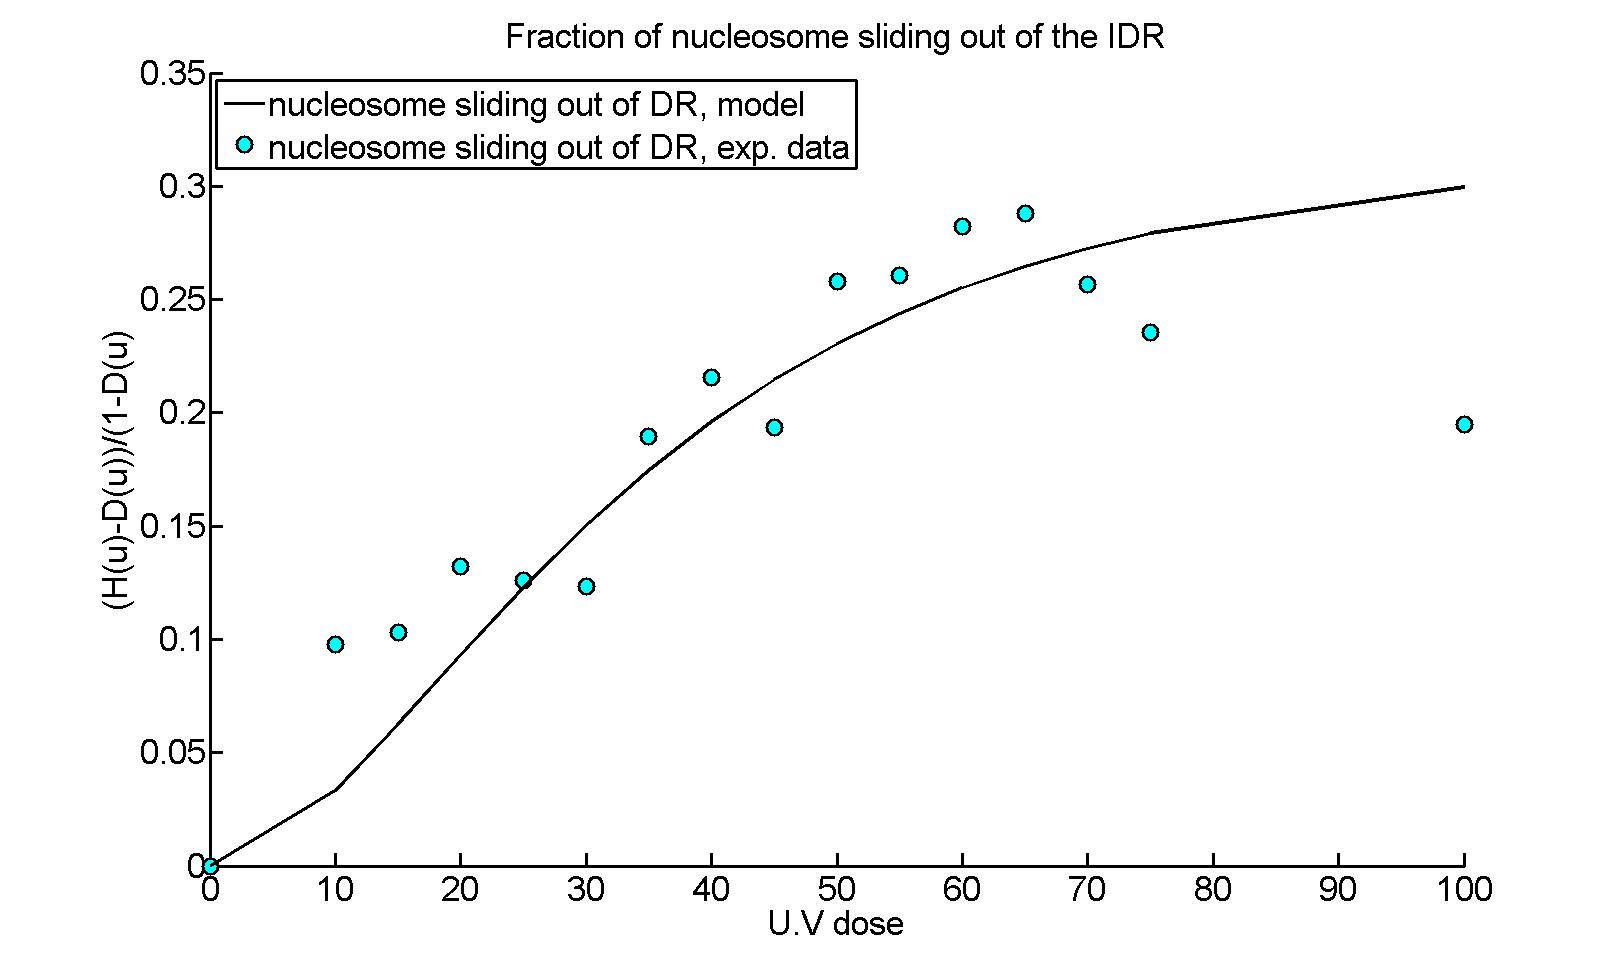
\includegraphics[width=0.5\linewidth, height=0.3\textheight]{fractionSlidingOutOfIDR}
\caption{\textbf{Fraction of nucleosomes sliding out of the IDR. The plot
		against the experimental data resulted in $R^2 = 0.75$}}
\label{fig:fractionSlidingOutOfIDR}
\end{figure}

The parameters values found in subsection \ref{subsection:parameterFit}, can further be used to estimate the fraction of nucleosome loss from the IDR attributed to sliding and
chromatin opening. These contributions are given by the leading coefficients
in the equations \eqref{eq:nucleosomePush} and \eqref{eq:nucleosomeSlide} for $N_P(u)$ and $N_S(u)$, respectively. We have, for
chromatin opening and sliding, respectively
\begin{equation*}
N_P(u) = 0.3N_T(u),\quad N_S(u) = 0.7N_T(u)
\end{equation*}

\end{document}